\documentclass[tufte-handout]{standalone}
\usepackage{mathpazo} % Sets Palatino as the main font
\usepackage{tikz}
\usetikzlibrary{3d, angles, quotes, calc, backgrounds}
\usetikzlibrary{decorations.markings}

% my colors
\definecolor{darkslategray}{rgb}{0.18, 0.31, 0.31}
\definecolor{myorange}{rgb}{0.89804, 0.55686, 0.19608}

\begin{document}

\begin{tikzpicture}

% Earth (Right)
\node[anchor=center] (earth) at (4, 0) {};
\draw[dashed, color=darkslategray, thick] (3.5, -2) -- (4.5, 2.25);
\node[anchor=center] at (4, 0) {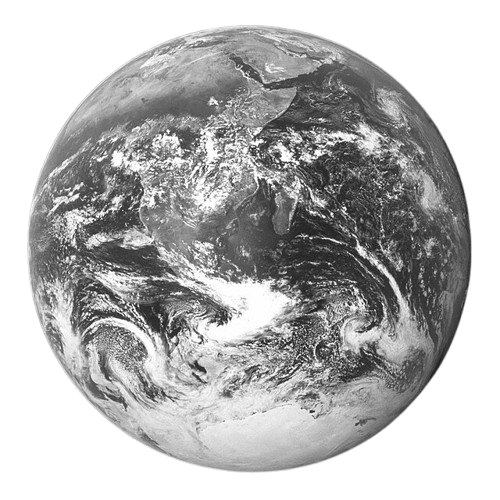
\includegraphics[width=3cm]{EarthImage.png}}; 
\node[anchor=west, xshift=0cm, yshift=-1cm, align=center] at  (0.15, 0.95) {\Large Terrestrial \\ \Large Detectors};
\begin{scope}[rotate=-15] % Adjust the rotation angle as needed
\draw[thick,->, color=darkslategray] 
    (4.15, 2.8) arc[start angle=45, end angle=-270, x radius=0.5cm, y radius=0.15cm];
\end{scope}
% Add your Earth texture here
\draw[myorange, fill=myorange] (3.75, 0.5) circle [radius=0.1cm];
\draw[myorange, fill=myorange] (3.8, 0.) circle [radius=0.1cm];
\draw[myorange, fill=myorange] (4.25, 0.05) circle [radius=0.1cm];
\draw[very thick, myorange] (3.75, 0.5) -- (3.8, 0.);
\draw[very thick, myorange] (3.8, 0.) -- (4.25, 0.05);

\draw[myorange, fill=myorange] (3.5, 0.2) circle 
[radius=0.1cm];
\draw[myorange, fill=myorange] (3.55, -0.3) circle 
[radius=0.1cm];
\draw[myorange, fill=myorange] (4, -0.25) circle 
[radius=0.1cm];
\draw[very thick, myorange] (3.5, 0.2) -- (3.55, -0.3);
\draw[very thick, myorange] (3.55, -0.3) -- (4, -0.25);


% Moon (Lower Left)
\node[anchor=center] (moon) at (-2, -2.5) {};
\draw[dashed, color=darkslategray, thick] (-2.4, -4.5) -- (-1.8, -0.5);
 \begin{scope}[rotate=-10] % Adjust the rotation angle as needed
    % Draw the curved arrow
    \draw[thick,->, color=darkslategray] 
        (-1.3, -1.2) arc[start angle=45, end angle=-270, x radius=0.5cm, y radius=0.15cm];
\end{scope}
\node[anchor=center] at (-2, -2.5){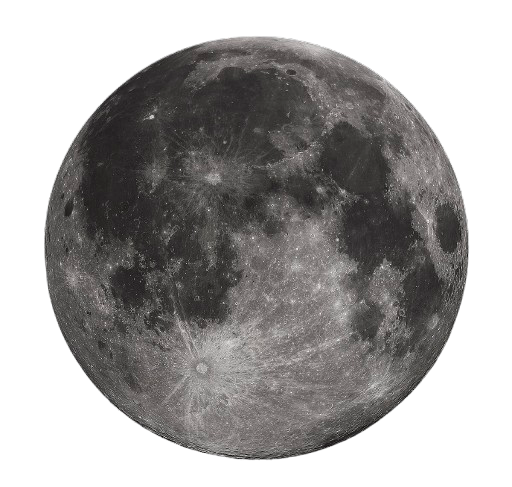
\includegraphics[width=3cm]{MoonImage.png}}; 
\node[anchor=west, xshift=0cm, yshift=-1cm, align=center] at  (-0.5, -1.5) {\Large Moon \\ \Large Detectors};
% Add Moon texture here
\draw[myorange, fill=myorange] (-2.5, -3.6) circle [radius=0.075cm];
\draw[myorange, fill=myorange] (-2.1, -3.7) circle [radius=0.075cm];
\draw[myorange, fill=myorange] (-2.275, -3.5) circle [radius=0.075cm];
\draw[myorange, fill=myorange] (-2.2, -3.25) circle [radius=0.075cm];

% Sun (Upper Left)
\node[anchor=center] (sun) at (0, 3) {};
\node[anchor=center] at (0, 3) {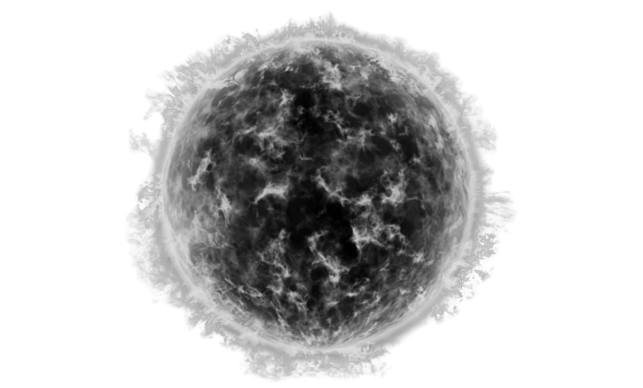
\includegraphics[width=3cm]{SunImage.png}}; % Add Sun texture here
% Tilted dashed ellipse
\node[anchor=east, xshift=0.5cm, yshift=0.2cm, align=center] at  (-2.05, 3) {\Large Space \\ \Large Detectors};
\draw[dashed, thick, rotate around={0:(0,3)}, color=darkslategray,decoration={
  markings,
  mark=at position 0.9 with {\arrow[scale=2]{stealth}} % Adjust the position (0.25) as desired
},
postaction={decorate}] (0,3) ellipse [x radius=4cm, y radius=1.5cm];

% Nodes
\node[circle, draw, color=myorange, fill=myorange, minimum size=0.1cm] (A) at (-1.5, 3.4) {};
\node[circle, draw, color=myorange, fill=myorange, minimum size=0.1cm] (B) at (-2, 0.9) {};
\node[circle, draw, color=myorange, fill=myorange, minimum size=0.1cm] (C) at (0.5, 1.8) {};


% Connections
\draw[very thick, darkslategray] (A) -- (B);
\draw[very thick, darkslategray] (B) -- (C);
\draw[very thick, darkslategray] (C) -- (A);

% Adjust the starting angles, ending angles, and radius as needed 
% so that the arc lies outside the triangle.
  
% For node A:
\draw[->, color=myorange, thick]
($(A)+(90:0.4)$) arc (90:180:0.4);

% For node B:
\draw[->, color=myorange, thick]
  ($(B)+(180:0.4)$) arc (180:270:0.4);

% For node C:
\draw[->, color=myorange, thick]
  ($(C)+(-30:0.4)$) arc (-30:60:0.4);

\node[anchor=center] at (-2.4, 1.8) {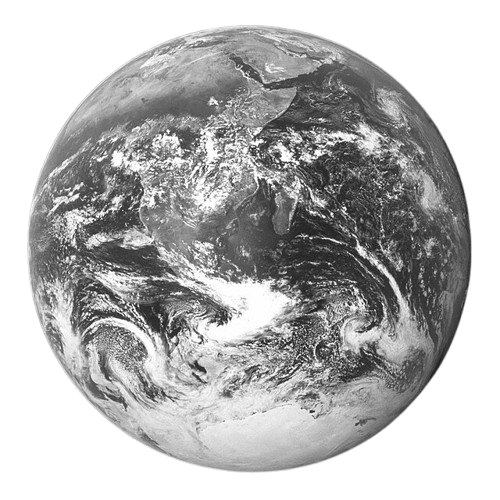
\includegraphics[width=0.25cm]{EarthImage.png}}; 

\end{tikzpicture}
\end{document}